\subsubsection{Anatomy and Physiology of Sense Organs}
\index{Meyer-Rochow, Victor Benno}


\paragraph{Research Team}
%
V. Benno Meyer-Rochow (Professor), Marina Zieger (Postdoc), Monalisa Mishra (PhD Student), Stanley T. Lau (PhD Student), Carsten HG M�ller (PhD Student), Dr Hans-Bert Schikora (Visiting Docent), Iikka Salmela (Part-time Lab Assistant)\\

The research carried out by us fell into three broad categories: (i) work related to comparative aspects of vision and other light-dependent phenomena, (ii) work related to life in the polar regions (i.e., the Antarctic and the Arctic), and (iii) work related to humans. There are, of course, overlaps and our theoretical study on the light-path in the eye of the Antarctic krill could be classified under headings (i) or (ii). Other research, like our electron microscopic work on the retinal fine-structures of beetles and centipedes or our publications on aspects of human health and welfare are more easily assignable to one of the categories. Principles that guide our research are ``comparative aspects'' and the importance of ``linkages'' between phenomena that, on occasion, seem little related to one another, but which, on closer inspection, often reveal numerous and exciting connections.

\paragraph{Highlights}
%
One of the highlights has clearly been the discovery through electrophysiological recordings from the eyes of live house centipedes (\textit{Scutigera coleoptrata}) that this crepuscular species not only has extraordinarily sensitive eyes, but that its spectral sensitivity peak lies in the UV at 350 nm wavelength. Another highlight was our paper on the unusual retinal organization and ultrastructure of a phylogenetically ancient centipede, the Tasmanian \textit{Craterostigmus tasmanianus}. Work in collaboration with scientists from Kalinigrad University (Drs. V. Zhukov, S.L. Borissenko, I.A. Vakoliuk) provided an example of the multipronged approach we are aiming for in all of our investigations of animal visual systems: light- and electron microscopy for structural elucidations, optical measurements and computer-assisted analyses to determine ray paths, and electrophysiological recordings and behavioural tests to investigate function. Two papers on invertebrate eyes that would be of interest to biologists active in applied fields were one that dealt with the juvenile eye structure and putative visual capacity in planktonic larval rock lobsters and a second one that investigated the photoreceptor organization in a species of beetle considered a pest on account of its habit to attack mushrooms.  A theoretical paper that presented a method to calculate the refractive index distribution in the dioptric systems of compound eyes of species that are difficult to obtain and/or impossible to transport alive to a laboratory equipped with an interference microscope, was published in the American ``Journal of Theoretical Biology'' and represented the 'fruit' of an international effort between Dr J. Gal in Hungary, Dr T. Miyazaki in Japan and Dr VB Meyer-Rochow at
IUB.\\
On the ``human health front'' several interesting results with inputs from our group to the Finnish coordinators of the research were published. Perhaps the most important of the findings is that contrary to the world-trend as well as WHO-data on suicides in the elderly (persons older than 65 years of age), in Finland this age-group displayed statistically significant lower incidences of suicides over a 15-year period than the age-group of the 18 - 65 year olds. Participation as an invited speaker at an Ethno-Entomology Symposium organized by Kyoto University is worth mentioning and so is the ongoing collaboration with Professor T. Hariyama and colleagues of Hamamatsu Medical University in Japan on functional aspects of rock lobster vision and extraretinal photoreception in fireflies.\\
Discussions with suicide researchers in Oulu (Finland) continued and saw a project emerge, which is led by Meyer-Rochow (i.e., suicides in visually-impaired people).\\
Another project that was started this year in collaboration with Korean scientists deals with the presence, significance, and origin of UV-patterns on the wings of butterflies and can be seen as an expansion of the current study of sexual eye dimorphism in insects, effects of UV-radiation on insect eyes, and phylogenetic relationships based on retinal ultrastructure. An examination of the eye of the commercially important slipper lobster (in collaboration with Prof. Ehud Spanier of Haifa University) has yielded first results and suggests high overall as well as polarization sensitivity for the eye of this crustacean. Finally, a highlight of a different sort was that even throughout the year 2006 our penguin publication of 2003 (Meyer-Rochow VB \& Gal J: Polar Biol. 27, 56-58) remained the most-viewed article of the ``Springer Verlag'' journal ``\textit{Polar Biology}''.


\begin{figure}[ht]
  \begin{center}
   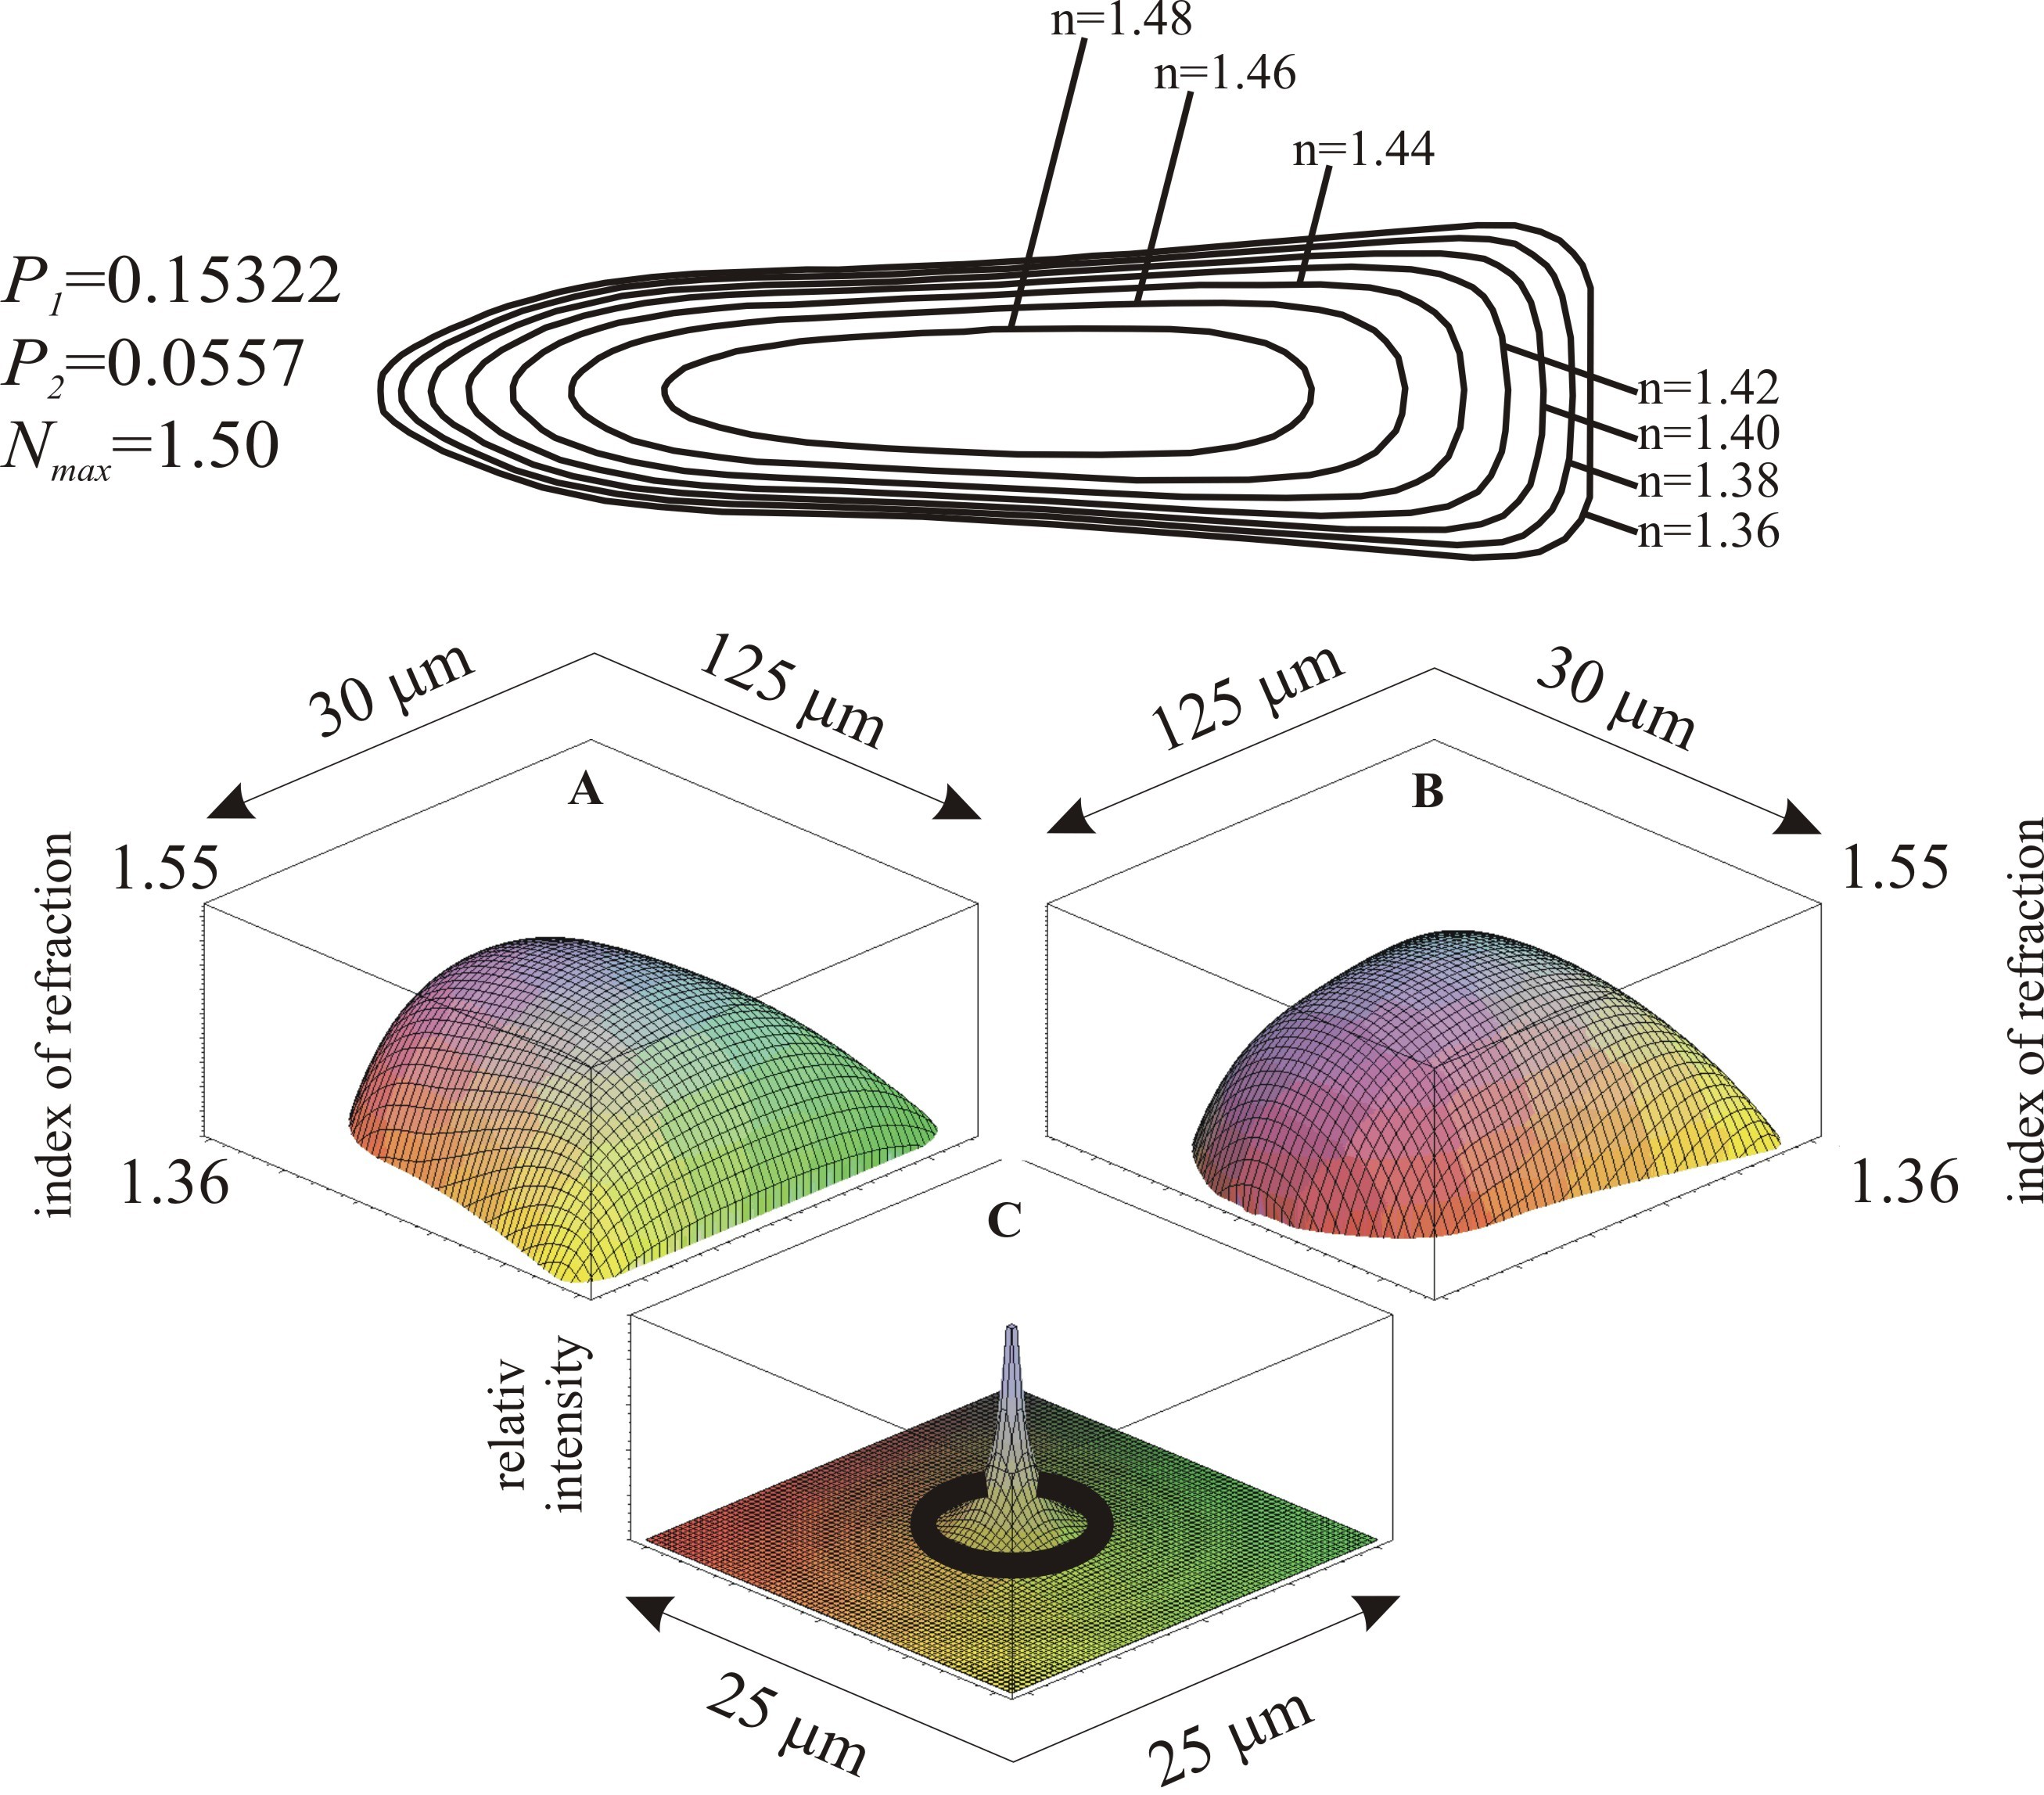
\includegraphics[width=\hsize]{Meyer-Rochow/Fig_Meyer-Rochow.jpg}
    \mycaption{ Calculated distribution of refractive index gradient in the crystalline cone of the Antarctic krill \textit{Euphausia superba} as 2D (A) and 3D  (B) representations. Distribution of light intensity on the distal retinal surface, calculated for the optimized model eye of E. superba is shown in (C) as a function of radial distance from the axis of the rhabdom. The black circle indicates the dimensions of a single rhabdom. For further information see Gal J, Miyazaki T, Meyer-Rochow VB: J. Theor. Biol., Vol.243 (2006).}\label{fig:Krill-FIG3}
   \end{center}
\end{figure}


\paragraph{Organization}
%
For his two months of research at Hamamatsu Medical University Meyer-Rochow received an invitation from the ``Society for the Promotion of Science'' in Japan.  The stays in Taiwan (one month) and South Korea (two months) were prompted by invitations from the Taiwan Academy of Sciences and Chonnam University, respectively.  Meyer-Rochow is one of the organizers of Hampyeong 2008 World Butterfly \& Insect Expo in South Korea.


\myparagraph{Collaborations}
%
Bremen Area Collaborations:
\begin{enumerate}
\item {\sl International University Bremen} \\ Prof.  A. Lerchl \\ Theoretical work on evolution of visual pigments
  \\ Prof.  M. Ullrich \\ Molecular taxonomy of mosses
\item {\sl University of Bremen} \\ Dr. H.-B. Schikora \\ New methods to trap small subterranean arthropods
\end{enumerate}
National \& International Collaborations:
\begin{enumerate}
\item {\sl University of Constance}\\ Dr. E. Gross \\Biological and micro-anatomical aspects of the water moth \textit{Acentria ephemerella}
\item {\sl Haifa University, Dept. of Marine Biology, Israel} \\Prof. E. Spanier\\ Eyes and vision in the slipper lobster
\item {\sl Helsinki University, Tv�rminne Zoological Station, Finland}\\ Dr. M. Lindstr�m \\ Electrophysiology of arthropod eyes
\item {\sl Oulu University, Fysiologian and Psykiatrian laitos, Finland}\\ O. Vakkuri \& M. Timonen\\Research into suicides, suicide ideation, and suicide risks
\item {\sl E�tv�s University ,Department of Biological Physics, Hungary}\\ Prof. G. Horvath and Drs. A. Barta and J. Gal \\ Polarization sensitivity of insect eyes
\item {\sl Kalinigrad University, Dept. of Ecological Physiology, Russia}\\ Prof. V. Zhukov\\ Retinal regeneration in amputated snail eyes
\item {\sl University of the West Indies, Electron Microscopy Unit, Jamaica}\\ Dipl.Ing. W.A. Reid \\ Eye ultrastructure in tropical insects
\item {\sl Medical University Hamamatsu, Dept. of Biology, Japan}\\ Prof. T. Hariyama \\ Sensory physiology of invertebrates
\item {\sl Yokosuka Natural History Museum (Japan) and National Taiwan University, Taiwan}\\    Dr. N. Ohba and Prof. E.C. Yang \\ Communication and defensive behaviour in fireflies
\item {\sl Fisheries Research Institute, Wellington, New Zealand}\\ Dr. A. Jeffs \\ Vision in larval rock lobsters
\item {\sl Federal University of Rio de Janeiro, Brazil}\\ Prof.  S. Allodi \\Vision in crustaceans
\end{enumerate}


\paragraph{Grants}
%
Research and travel grants were received 1. from Oulu University (Finland) for research with Prof. Gabor Horvath on polarizing properties of insect cuticle, 2. from the Academy of Sciences of Taiwan for work on beetle luminescence, 3. from The Society for the Promotion of Science in Japan for research on sensory physiological aspects of invertebrates, 4. from Chonnam University and the Hampyeong Gun Insect Institute of South Korea for helpimng to organize the 2008 Butterfly \& Insect World Expo, and 5. from the Socrates/Erasmus Programme to teach second year medical students at Oulu University (Finland). Some assistance for a student's visit to Israel was obtained from Haifa University (Israel) to work on the organization and fine structure of dark- and light-adapted slipper lobster eyes.



\nocite{Meyer-Rochow1,Meyer-Rochow2,Meyer-Rochow3,Meyer-Rochow4,Meyer-Rochow5,Meyer-Rochow6,Meyer-Rochow7,Meyer-Rochow8,Meyer-Rochow9,Meyer-Rochow10,Meyer-Rochow11,Meyer-Rochow12,Meyer-Rochow13,Meyer-Rochow14,Meyer-Rochow15,Meyer-Rochow16,Meyer-Rochow17,Meyer-Rochow18,Meyer-Rochow19,Meyer-Rochow20}
